\documentclass[11pt,a4paper]{article}
\usepackage[latin1]{inputenc}
\usepackage{steinmetz}
\usepackage{gensymb}
\usepackage{amsmath}
\usepackage{amsfonts}
\usepackage{amssymb}
\usepackage{graphicx}
\author{Jordan Murray}
\title{EECS305 Lab4}
\begin{document}
\begin{center}
\fontsize{24}{12}\selectfont
\textbf{Lab 4: Lead-Lag Control of a DC Servo Motor}
\end{center}
\section{OBJECTIVES}
\begin{enumerate}
\item To understand the concept of system type and its implication on tracking ability.

\item To design a lead-lag compensator for a DC servo motor system.

\item To analyze the transient response of the system with or without lead-lag compensators.
\end{enumerate}

\section{BASIC KNOWLEDGE}
In this experiment, we introduce mathematical models for a DC servomechanism and lead-lag compensator design using the root-locus method

A block diagram for a typical servomechanism is shown in Fig. ~\ref{fig:servoblock}.  The action of the servomechanism is to track a desired position (or speed) despite the 
presence of disturbance inputs to the system and errors in the 
sensor data.

\begin{figure}[here]
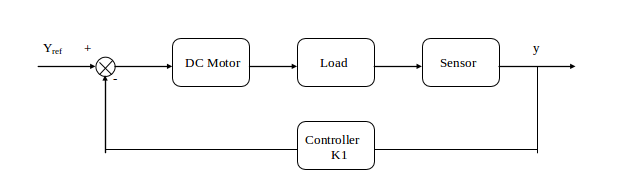
\includegraphics[width=\textwidth]{imglab/servoblockdiagram.png}
\caption{Servomechanism block diagram}
\label{fig:servoblock}
\end{figure}

\subsection{Model Development}
\begin{figure}[here]
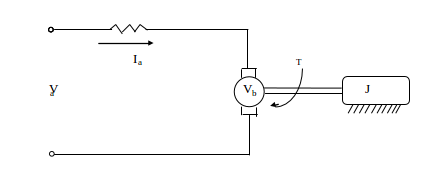
\includegraphics[width=\textwidth]{imglab/servoschemdiagram.png}
\caption{schematic diagram of the DC servo motor}
\label{fig:servoschem}
\end{figure}

We begin by developing a simplified linear model of an armature controlled DC servo motor and load. Fig. ~\ref{fig:servoschem} shows the schematic diagram of the motor and load.

Neglecting the inductance of the armature circuit, the armature voltage V$_{a}$ produces a current I$_{a}$ as given by:

\begin{equation} \label{eq:1}
I_{a}(t) = \frac{V_{a}(t)-V_{b}(t)}{R_{a}}
\end{equation}

Here V$_{b}(t)$ denotes the back emf of the motor and R$_{a}$ is the armature resistance.

The motor torque $T(t)$ is proportional to I$_{a}(t)$:

\begin{equation} \label{eq:2}
T(t) = K_{T}I_{a}(t)
\end{equation}

From Newton's law, assuming an inertia load:

\begin{equation} \label{eq:3}
T(t) = J\ddot{\theta}(t)
\end{equation}

combining equations \ref{eq:1}, \ref{eq:2}, and \ref{eq:3} we obtain:

\begin{equation} \label{eq:4}
K_{T}\left[\frac{V_{a}(t)-V_{b}(t)}{R_{a}}\right] = J\ddot{\theta}(t)
\end{equation} 

Using the relationship V$_{b}$ = K$_{b}\dot{\theta}$ and, letting V$_{a}(t)$ = u(t) (the input signal), we have:

\begin{equation} \label{eq:5}
\frac{K_{T}}{R_{a}}\left[u(t)-K_{b}\dot{\theta}(t)\right] = J\ddot{\theta}(t)
\end{equation}

\begin{equation} \label{eq:6}
\frac{JR_{a}}{K_{T}}\ddot{\theta}(t)+ K_{b}\dot{\theta}(t) = u(t)
\end{equation}

\begin{equation} \label{eq:7}
\ddot{\theta} + \frac{K_{b}K_{T}}{JR_{a}}\dot{\theta} = \frac{K_{T}}{JR_{a}}u(t)
\end{equation}

or letting $\omega$(t) = $\dot{\theta}(t)$, and 

\begin{equation} \label{eq:8}
\dot{\omega}(t) + \frac{K_{b}K_{T}}{JR_{a}}\omega(t) = \frac{K_{T}}{JR_{a}}U(t)
\end{equation}

Equations \ref{eq:7} and \ref{eq:8} are the differential equations for the DC motor.

Let $\frac{K_{b}K_{T}}{JR_{a}} = \frac{1}{\tau}$, $\frac{K_{T}}{JR_{a}} = \frac{K_{0s}}{\tau}$. Here, $K_{s}$ is the static gain and $\tau$ is the time constant of the system. The D.E. \ref{eq:7} is a model of the system from the input voltage to the output speed. Using the Laplace transform we can convert to the following transfer function from input ($u(t)$) to output position ($\theta (t)$:

\begin{equation} \label{eq:9}
\frac{\Theta(s)}{U(s)} = \frac{K_{s}}{s(\tau s + 1)}
\end{equation}

From the D.E. \ref{eq:8} the transfer function of the DC motor from input $u(t)$ to output speed $\dot{\theta}(t)=\omega(t)$ is:

\begin{equation} \label{eq:10}
\frac{\Omega (s)}{U(s)} = \frac{K_{s}}{(\tau s + 1)}
\end{equation}

The system can be depicted as in Fig. ~\ref{fig:servomeasschem}

\begin{figure}[here]
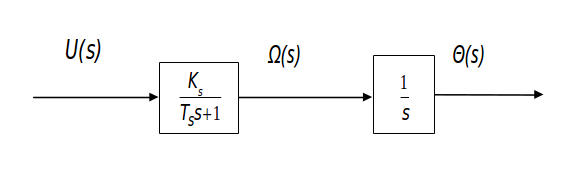
\includegraphics[width=\textwidth]{imglab/servoschematicnomeasurement.png}
\caption{Schematic of the DC servo system}
\label{fig:servomeasschem}
\end{figure}

The model from input armature voltage to output position has one pole at the origin and one pole on the negative real axis. The problem is to identify the parameters $K_{s},and \tau$. The transfer function from input $u(t)$ to output $\theta(t)$ is:

\begin{equation} \label{eq:11}
\frac{\Omega(s)}{U(s)} = \frac{K_{s}}{\tau s + 1}
\end{equation}

The unit step response of the first order system is shown in Fig. ~\ref{fig:servostepresp}:

\begin{figure}[here]
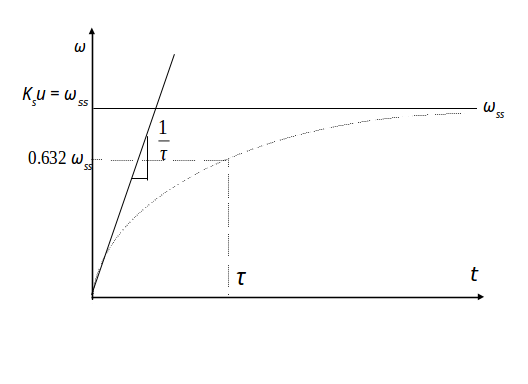
\includegraphics[width=\textwidth]{imglab/servostepresponse.png}
\caption{step response of the DC servo motor}
\label{fig:servostepresp}
\end{figure}

From this response, we can determine that the time constant of the motor, $\tau$, is the time it takes $\omega(t)$ to reach 63.2\% of its steady-state value $\omega_{ss}$. We can also obtain the steady-state gain $K_{s} = \frac{\omega_{ss}}{u_{ss}}$.

\subsection{Closed-Loop Control for a DC servomechanism} \label{ss:closedloop}
The block diagram of Fig. ~\ref{fig:servoblock} for the servomechanism can be simplified into the block diagram given in Fig. ~\ref{fig:servotfblock}.

\begin{figure}[here]
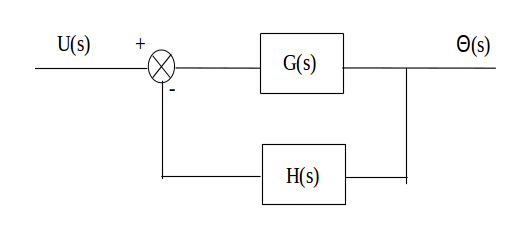
\includegraphics{imglab/servotfblock.png}
\caption{Simplified block diagram}
\label{fig:servotfblock}
\end{figure}

This configuration is referred to as a negative feedback closed-loop control system where $G(s)$ is the forward loop transfer function and H(s) is the feedback loop transfer function. The equivalent transfer function between the input r(t) and the output c(t) as shown in Fig. ~\ref{fig:servostepresp} can be represented as the transfer function $G^{\prime}(s)$ shown in Fig. ~\ref{fig:servocltfblock}.

\begin{figure}[here]
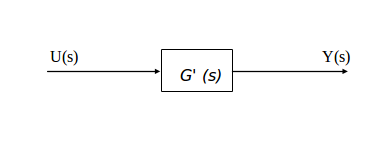
\includegraphics{imglab/servocltfblock.png}
\caption{Equivalent closed-loop transfer function}
\label{fig:servocltfblock}
\end{figure}

\begin{equation} \label{eq:15}
G'(s)=\frac{Y(s)}{U(s)}=\frac{G(s)}{1+G(s)H(s)}
\end{equation}

Considering the servomechanism transfer function:

From Eq. \ref{eq:9}: $G(s)=\frac{K_{s}}{s(\tau s + 1)}$,

H(s) = K$_{1}$ (Output feedback controller gain),

\begin{equation} \label{eq:12}
G'(s)=\frac{\frac{K_{s}}{\tau}}{s^{2} + \frac{s}{\tau} + \frac{K_{1}K_{s}}{\tau}}
\end{equation}

We observe that the transfer function of the closed-loop system, $G^{\prime}(s)$, is a second order system with one free controller parameter $K_{1}$. Changing the gain $K_{1}$ can be used to alter the transient response dynamics of the closed-loop second order system.


\subsection{Background information on lead-lag compensator design}
Lead and lag compensators are used quite extensively in control. A lead compensator can increase the stability or speed of response of a system; a lag compensator can reduce (but not eliminate) the steady state error. If improvements in both transient response and steady-state response are desired, then both a lead compensator and a lag compensator may be used simultaneously. Depending on the effect desired, one or more lead and lag compensators may be used in various combinations.

%\subsubsection{Lead compensator}

%\subsubsection{Lag compensator}

\section{EXPERIMENTAL PROCEDURES}

\subsection{System Type and Tracking Error}
In this portion of the procedure, we explore the effect of system type on our ability to track reference signals of various types. The Simulink model used in this portion includes five different cases. First, we have position feedback used to track a step, ramp, and parabolic reference. The remaining two cases use speed feedback with step and ramp references. 

Procedure:
\begin{enumerate}
\item Open the model \textbf{Lab4\_SystemType.slx} and run it. For each case, observe the following: Does the system state track the reference? If not, characterize the error (is the error constant, increasingly linearly, increasing quadratically, etc.). How does the system's ability to track the same signal differ depending on whether speed or position is being tracked?

\item If a reference signal is not being tracked, adjust the gain for that case. What happens to the error? Is it possible to eliminate the error?
\end{enumerate}

\subsection{Identify $K_{s}$ and $\tau$}
\begin{enumerate}
\item Run MATLAB and open the model \textbf{Lab4\_identification.slx}. The DC servo block contains a masked model of a DC servo motor. Run the model. A unit step input is applied to the motor winding at t = 1s. Open the scope and look at the angular velocity trace. Determine the steady-state speed of the motor. This is the value of $K_{s}$, the steady-state gain. Determine the time at which the speed reaches 63.2\% of its final value. Find the elapsed time since the step function was applied. This value is the time constant $\tau$.
 
\end{enumerate}



%\subsection{Lag Compensator Design}
%We want a lag compensator that will affect our transient response as little as possible, but will increase steady-state gain. As such, we want our pole and zero to very close to each other (consider the angle and magnitude criteria), but we also want the ratio of zero to pole to be large enough to achieve the desired steady-state gain. Both  of these requirements can be achieved if we place the zero and pole for the lag compensator near the origin. 

%Suggested procedure:
%\begin{enumerate}
%\item Place the zero to the right of the real projection of the lead compensated system's closed loop pole by a factor of 50-100.
%\end{enumerate}


\subsection{Proportional Feedback}
\begin{enumerate}
\item Open the Simulink model \textbf{Lab4\_ProportionalFeedback.slx}, which contains our servo model with fixed gain feedback. 

\item What is the shortest settling time you can obtain with proportional feedback that results in a peak overshoot of less than 5\%? You might use MATLAB's rlocus() to plot the root locus, sgrid() to get the boundary associated with our zeta constraint, and rlocfind() to get the gain associated with your desired closed loop pole locations.

\end{enumerate}

\subsection{Designing a Lead Compensator for Better Performance}
\begin{enumerate}


\item We know system parameters $K_{s}$ and $\tau$, with which we can estimate the transfer function of the motor and design a controller accordingly.

\item The transient response specifications are as follows:
\begin{enumerate}
\item Maximum percentage overshoot less than 5%
\item Settling time (2\% band) less than .6 seconds
\end{enumerate}

Calculate the corresponding restrictions on the values of the damping ratio $\zeta$ and the natural frequency $\omega_{n}$.


\item Determine our desired closed loop dominant pole locations from the $\zeta$ and $\omega_{n}$ calculated in the previous step. You might try selecting the points at the intersections of the constraining curves from the previous step.

\item  The open loop system consisting of the controller and plant has 1 zero and 3 poles. The open loop plant poles are fixed at zero and 1/$\tau$. The compensator pole and zero must be chosen so that the root locus intersects the desired pole location. The feedback gain associated with this point on the root locus must then be determined. \textit{You will have to show this work in your report.}

Suggested procedure:
\begin{enumerate}

\item Find the real axis projection of the desired pole location.

\item \label{step:zeropos} Place the controller zero at or to the left of this point on the real axis, but not too far (consider the limit in which the lead pole goes to $-\infty$ and has an angle of 0).

\item Determine where on the real axis the controller pole must be placed using the \textit{angle criterion}. Remember that a lead compensator has its pole to the left of its zero.

\item If no valid angle can be found, go back to step \ref{step:zeropos} and choose a different zero location.

\item Find the feedback gain. You might use the \textit{magnitude criterion} and check your result with the matlab command rlocfind(). 

\end{enumerate}

\item Record the zero, pole, and gain values.

\item Open the Simulink model \textbf{Lab4\_Lead.slx}. This model contains the following five systems:

\begin{center}
\begin{tabular}{|c|c|c|c|c|c|c|c|}
\hline
System & Input & Control  \\ \hline
1 & step & lead in feedback path \\ \hline 
2 & step & lead in forward path \\ \hline 
3 & ramp & lead in feedback path \\ \hline 
4 & ramp & lead in forward path \\ \hline 
5 & ramp & proportional \\ \hline 
\end{tabular}
\end{center}


\item For systems 1-4, change the gains and lead compensator transfer function blocks to match the controller parameters just determined. For system 5, set the G5 block to a proportional gain constant determined in the previous part, or another value that meets the maximum overshoot constraint.

\item Run the simulation. 

Regarding the step-fed systems, does the system trajectory meet the specifications? How do the responses of the feedback path compensated system and the forward path compensated system differ? What impact does the compensator configuration have on the closed loop transfer function and how does this explain the transient behavior?

Regarding the ramp-fed systems, how does the lead compensator and its placement affect the steady state error?

\end{enumerate}

%\subsection{Lag Compensation}
%\begin{enumerate}
%\item Open the Simulink model \textbf{Lab4\_Lag.slx}, which contains our servo model with a lag compensator transfer function in the forward path.

%\item Plot the root locus of the lag compensated system.

%\item Try and find a gain that does not exceed our overshoot limit of 5\%. What is the settling time? What is the effect of the lag compensator on the root locus and the resultant transient behavior.

%\end{enumerate}

\subsection{Lead-Lag Compensation: Transient Performance with Steady-State Error Reduction}
Using a lag compensator in addition to a lead compensator can reduce steady state error without significantly changing the transient behavior. We will now design a lag compensator to be used along with the lead compensator from a previous section to improve the ability of the DC servo system to track a ramp reference.

To our overshoot and settling time restrictions, we now add the following requirements:

\begin{enumerate}
	\item A steady state velocity error when subject to a unit ramp input of less than .02.
	\item Approach this error quickly without significant detriment to the transient performance.
	
\end{enumerate}

\begin{enumerate}

\item Design the lag compensator. You might use the following procedure.

\begin{enumerate}

\item Determine $K_{v}$ from the steady state speed error requirement.

\item For a lag compensator $\frac{s+\frac{1}{T}}{s+\frac{1}{\beta T}}$, determine $\beta$ using the relation $K_{v} = \lim_{s \to 0} s K G_{lead}(s) G_{lag}(s) G_{servo}(s)$ to achieve the target $K_{v}$. K is the lead compensator gain.

\item Determine T such that 

\begin{equation}
\lvert \frac{s_{1}+\frac{1}{T}}{s_{1} + \frac{1}{\beta T}} \rvert \approx 1
\end{equation}

\begin{equation}
-5 \degree < \phase{\frac{s_{1}+\frac{1}{T}}{s_{1} + \frac{1}{\beta T}}} < 0 \degree
\end{equation}

where $s_{1}$ is one of the closed loop pole locations.

\end{enumerate}

\item Open the Simulink model \textbf{Lab4\_LeadLag.slx}. This model contains two step input systems for comparing transient behavior between the lead and lead-lag compensated systems. Two ramp input systems are also included for observing the difference in steady state velocity error between the lead and lead-lag compensated systems.

\item Modify the lead and lag compensator transfer function  and gain blocks to reflect the correct controller parameters.

\item Run the simulation.

\item Confirm that the transient response of the step-input system is almost the same as before the addition of the lag compensator.

\item Look at the ramp input systems. Compare the error of the lead compensated system to that of the lead-lag compensated system. Does the lag compensator reduce the steady state error to the level required? How long does it take for the desired error tracking performance to be attained?

\end{enumerate}



\section{REPORT}

\begin{enumerate}

\item Explain the tracking errors observed in the System Type and Tracking Error section in terms of the Final Value Theorem.

%\item Plot the transients responses from \ref{ss:transient}. Compare the results of the three situations. Comments are needed to describe the effects of the lead compensator and lag compensator and illustrate why they have those effects.

%\item Consider the transient responses observed in \ref{ss:transient} for the constant feedback, lead compensated, and lag compensated cases. Comment on the effects of each controller in the time domain and on the locations of the closed loop poles. Explain the reasons for these effects in terms of the open loop zeros (if any) and poles and the feedback gain.

%\item Show the detailed procedure of designing the lead compensator based on the root-locus approach. What parameters did you determine for the servo motor? What values did you calculate for $\zeta$ and $\omega_{n}$? What about the zero and pole locations and the gain for the lead compensator? Were you able to meet the specifications laid out in ~\ref{ss:specs}?




\end{enumerate}

\end{document}
